\documentclass{article}

% NeurIPS 2026 Evaluations & Datasets track submission format.
\PassOptionsToPackage{numbers,compress}{natbib}
\usepackage[eandd]{neurips_2026}

\usepackage[utf8]{inputenc}
\usepackage[T1]{fontenc}
\usepackage{graphicx}
\graphicspath{{figures/}}
\usepackage{hyperref}
\hypersetup{
  colorlinks=true,
  linkcolor=black,
  citecolor=black,
  urlcolor=black,
  pdfborder={0 0 0}
}
\usepackage{url}
\usepackage{booktabs}
\usepackage{multirow}
\usepackage{amsfonts}
\usepackage{amsthm}
\usepackage{nicefrac}
\usepackage{microtype}
% \usepackage{xcolor}
\usepackage[dvipsnames]{xcolor}

\newcommand{\note}[1]{\colorbox{BurntOrange}{(#1)}}

\newtheorem{lemma}{Lemma}
\newtheorem{proposition}{Proposition}
\newtheorem{corollary}{Corollary}
\title{Determining optimal training strategies using cross-validation with subsets and downsampling}
\author{Anonymous}

\begin{document}

\maketitle

\begin{abstract}
In many machine learning applications, data come with subsets defined by geography, time period, acquisition protocol, demographic group, etc.
% Previous methods for estimating generalization error 
When model performance differs across subsets of different sizes, we would like to determine the cause (number of train data, or distributional difference between subsets).
% If the gap reflects unequal training-set sizes, more data collection is needed; if it reflects genuine distributional differences, domain adaptation or robustness methods are needed.
% Standard cross-validation and the SOAK framework \citep{hocking2026} do not separate these two causes.
We propose SOKED (Same/Other K-fold cross-validation Extension: Downsampling), a new machine learning evaluation framework that formally decomposes an observed performance gap into a \emph{sample-size component} and a \emph{residual subset component} by using matched-size downsampling to equalize training set sizes.
% The decomposition can reverse the apparent ordering of training configurations: in our experiment on the dataset "workers' compensation", the naive full-data comparison suggests Other training data is superior, while SOKED shows the gap is not significant once training-set size is controlled.
After size matching, subset advantages either disappear (indicating a sample-size effect; subsets are compatible), or persist (indicating a true distributional difference between subsets), depending on the data set.
% , so domain adaptation methods may be required for optimal learning and prediction).
We show the advantages of the proposed SOKED framework relative to baselines, using simulations and real data sets from diverse domains: traffic monitoring, insurance claims, image classification, survey data, and microbial biogeochemistry.
% We implement SOKED in the \texttt{mlr3resampling} R package.
\end{abstract}


\section{Introduction}
In many real-world machine learning problems, the data fall into natural subsets defined by time period, geographic region, collection protocol, demographic group, etc.
When model performance differs across these subsets, it is not obvious whether the difference comes from genuine heterogeneity in the data or from the simpler fact that some subsets contain more training examples than others.

For example, consider creating a public health monitoring system using data from the National Survey of Children’s Health \citep{NSCH2019}, which contains subsets for different years of data collection (18,202 survey responses in 2019 and 27,808 in 2020).
In the previous SOAK evaluation framework \citep{hocking2026}, we fix a test subset (2020), then systematically compare models trained using data from either the same year (2020), or from the other year (2019). 
If the model trained on the same year performs better than the model trained on the other year, is this improvement because there are more training examples (sample size effect), or because the other year has a different data distribution (subset effect) that makes learning and prediction more difficult?
% If the gain comes solely from the sheer data volume, then the practical response is to combine years when training. 
If real distributional shifts exist between years, then separate models can be trained for each year, or data can be combined using domain adaptation techniques \citep{CostaJussa2015}.
However, the previous SOAK framework does not separate subset effects (distributional differences) from sample-size effects (performance gains due to more training data), so its conclusions can be misleading when subsets differ substantially in size.

We propose SOKED (\textbf{S}ame/\textbf{O}ther/\textbf{A}ll \textbf{K}-fold cross-validation \textbf{E}xtension: \textbf{D}ownsampling), a new evaluation framework that formally decomposes an observed performance gap into a \emph{sample-size component} and a \emph{residual subset component}.
By holding training set size fixed through matched downsampling, SOKED empirically estimates the cause of performance differences: either a sample-size effect (the ordinary benefit of more training data) or a subset effect (genuine differences in learnable patterns between subsets).
% The decomposition changes the recommended action: a sample-size effect calls for collecting more data, while a residual subset effect calls for distributional robustness methods or domain adaptation.

% The decomposition can also reverse the apparent ordering of training configurations and expose a failure mode of naive full-data comparison.
% In our experiment on the dataset "workers' compensation", the full-data comparison favors the Other model for female subset; after size-matching, SOKED shows the gap shrinks to non-significance ($p > 0.1$), revealing that the apparent advantage is largely explained by training-set size rather than a genuine distributional difference.
% We demonstrate this and related phenomena across simulated regression, benchmark classification (STL-10, Waveform), epidemiological survey data (NSCH autism), and microbial biogeochemistry (qSIP).

\textbf{Summary of contributions.}
We present three contributions.

\textbf{1. New SOKED evaluation framework and software gap.}
  We propose SOKED, a new evaluation framework which uses downsampling to distinguish sample-size effects from residual subset effects.
  To our knowledge, no prior software implements this Same/Other diagnostic with matched-size comparisons, so SOKED fills a practical software gap for cross-validation over predefined subsets.

  
\textbf{2. Mathematical analysis.}
  We introduce a decomposition of cross-validation performance gaps into a sample-size component and a residual subset component, using matched-size downsampling.
  Lemma~\ref{lem:exchangeability} gives a sufficient condition under which the subset component is zero.

\textbf{3. Benchmark file format and empirical demonstrations.}
  We propose a simple standard file format for benchmarking Same/Other subset comparisons and release eight datasets in that format.
  % Each benchmark file makes the resampling splits, subsets, target, and predictors explicit using \texttt{fold}, \texttt{subset}, \texttt{y}, and \texttt{x} columns.
  We use these data to highlight the novelty of the proposed SOKED algorithm, which separates apparent advantages caused by unequal training-set sizes from residual subset effects that persist after size matching.


\section{Related work}

\textbf{Cross-validation and model validation.}
Cross-validation is a standard tool for model assessment \citep{stone1974cross,geisser1975predictive,Arl_Cel:2010:surveyCV} embedded in modern benchmarking frameworks such as \texttt{mlr3} and \texttt{origami} \citep{Bischl2024,coyle2018origami}.
Structured resampling methods account for spatial, temporal, or hierarchical dependencies by blocking or grouping observations \citep{roberts2017,brenning2005,valavi2019,schratz2024}.
These mechanisms control how folds are formed; SOKED answers a different question: after the split is fixed, which subset should supply the training examples, and how much of any observed performance gap is due to training-set size against genuine distributional differences?

\textbf{Distribution shift and transfer learning.}
Transfer learning and domain adaptation methods are prescriptive: given a distributional shift, they adapt a source model to a target domain \citep{pan2010transfer,Farahani2021}.
The proposed SOKED framework is instead diagnostic: it determines whether same-subset or other-subset training data are more predictive for a fixed target subset, and decomposes any gap into a sample-size component and a residual subset component.
The previous SOAK framework includes a comparison with training on all subsets, but does not include downsampling, so is not able to determine the cause of performance differences when training on subsets of unequal sizes \citep{hocking2026}. 
The proposed SOKED framework focuses on the Same/Other contrast and proposes a new downsampling method to handle the practically important case of unequal subset sizes.

\textbf{Fairness auditing.}
Demographic subgroups are often imbalanced in size, so an observed performance disparity may reflect either genuine distributional differences or simply less training data for the disadvantaged group \citep{savoldi2021gender,hall2024visogender}.
SOKED separates these two causes: a sample-size finding calls for targeted data collection, while a residual subset effect calls for bias mitigation strategies.

\section{Methods}

\begin{figure}
    \centering
    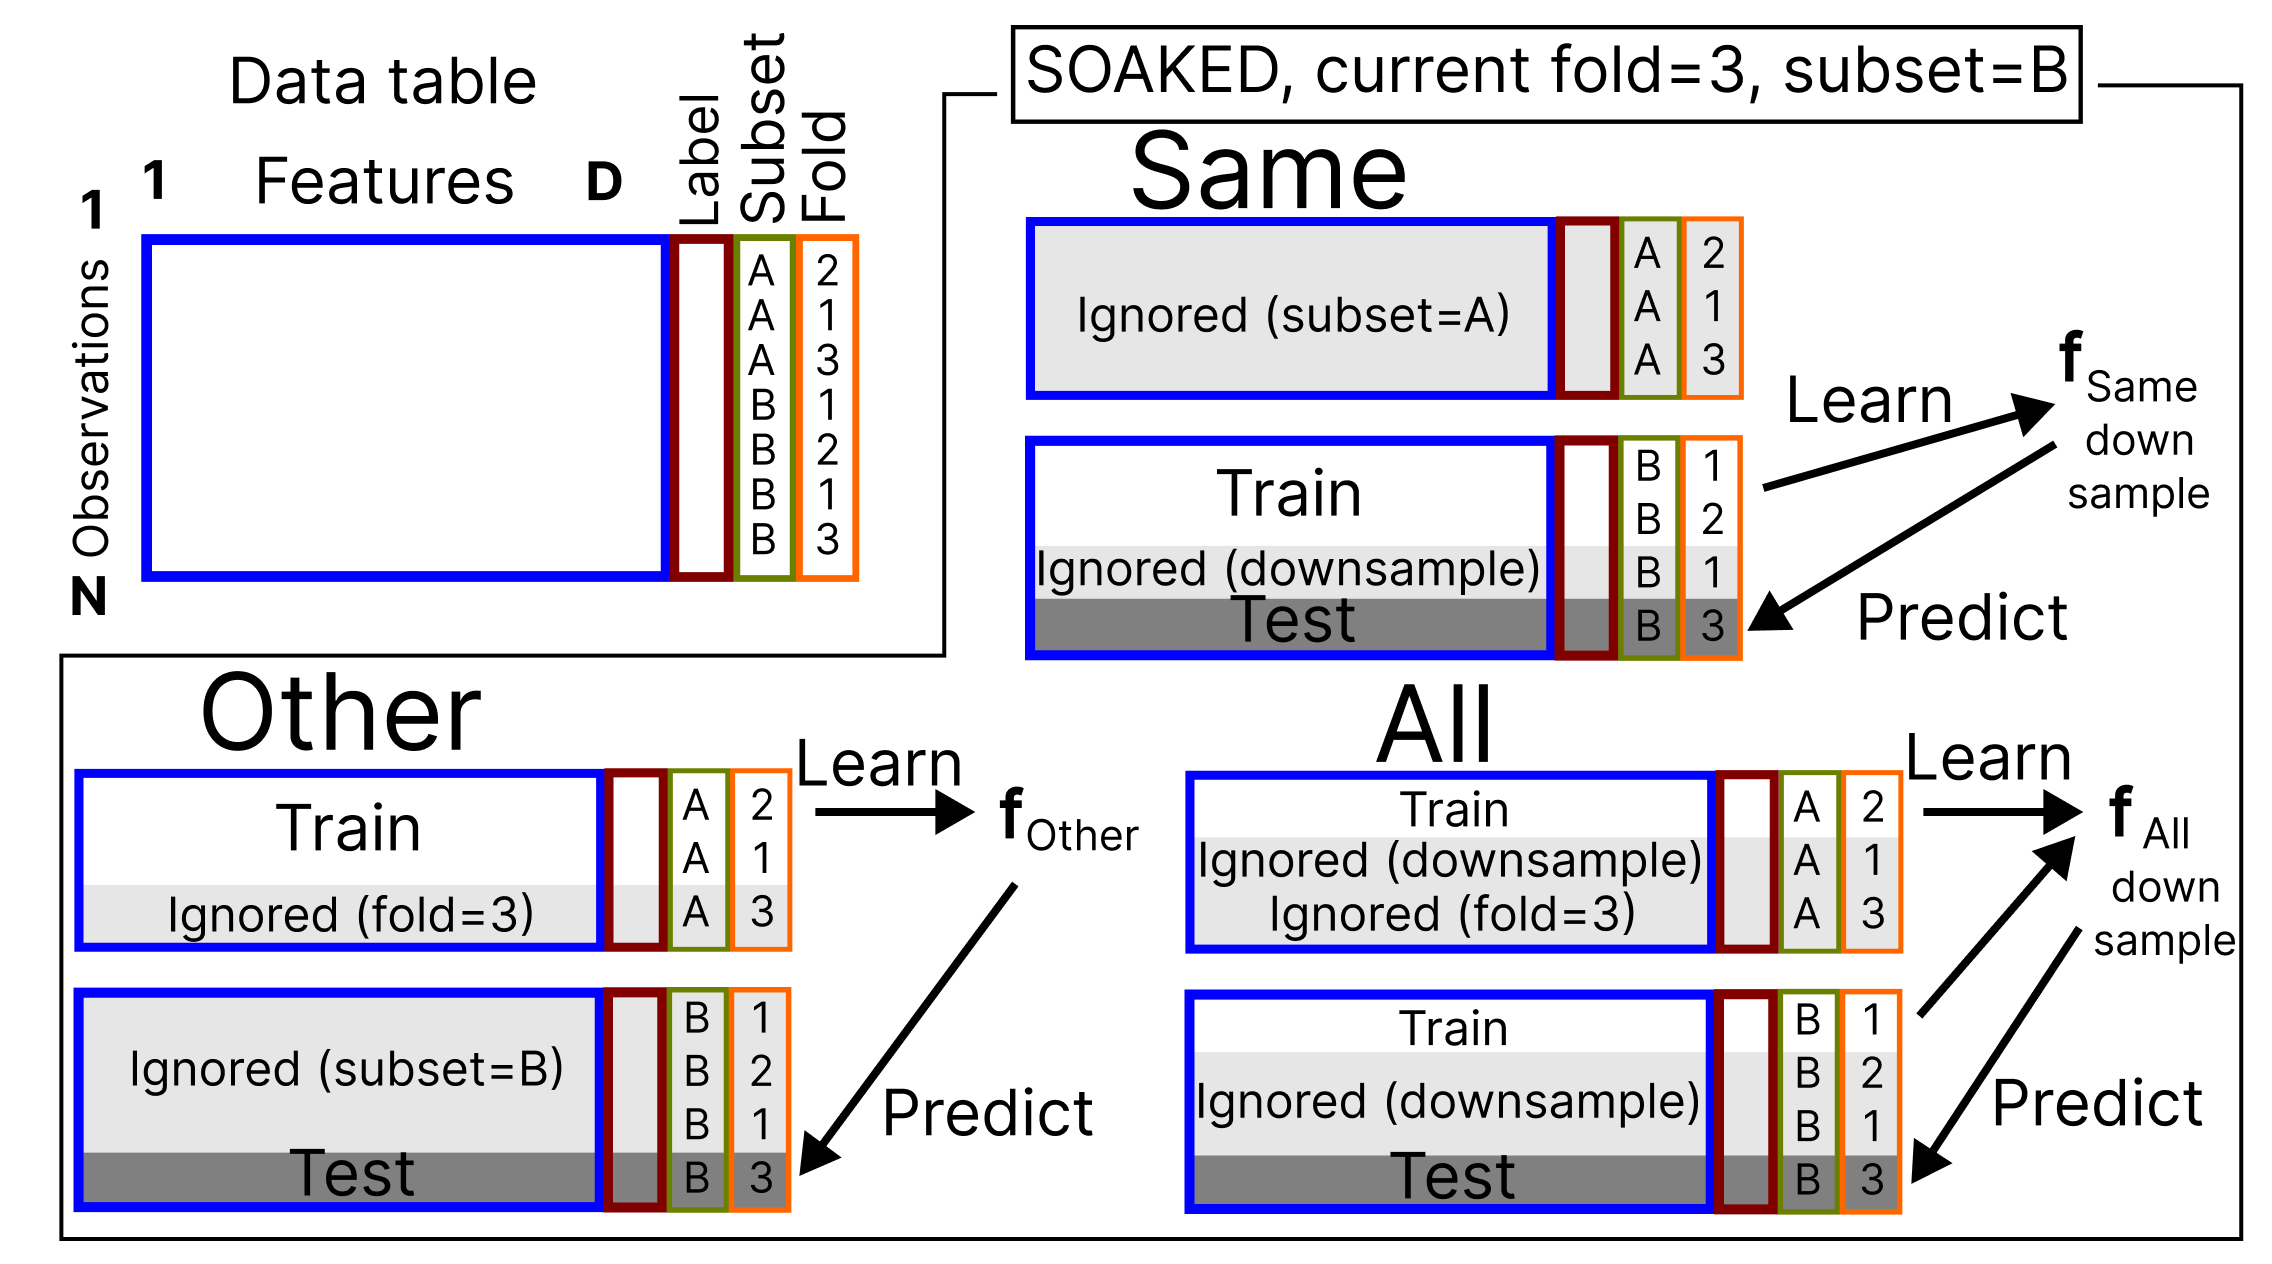
\includegraphics[width=1\linewidth]{fig1-concept.png}
    % https://github.com/tdhock/cv-same-other-paper/blob/main/slides/drawing-SOKED-generic.svg
    \caption{
    Proposed SOKED evaluation framework, for test fold=3 and test subset=B, in data with two subsets of different sizes: A has three rows and B has four rows.
    After excluding data based on fold and subset, random downsampling is used to obtain train sets of size equal to the smaller train set (Other, 2 rows).}
    \label{fig:SOKED-concept}
\end{figure}

\subsection{Proposed SOKED evaluation framework}
\label{sec:workflow}
The goal of the proposed SOKED method is to determine if data subsets are similar enough for optimal learning and prediction.
% We fix a test fold and a target subset, then compare predictors trained on either the Same subset, or the Other subset.
% SOKED retains both the original full-data training sets and matched-size versions obtained by random downsampling to the smaller feasible training set, so the full-data gap and the size-controlled gap can be compared.
% For one target subset, SOKED proceeds as follows.
\begin{enumerate}
    \item \textbf{Fix the test subset.} Choose the target subset whose test performance will be evaluated.
    \item \textbf{Analyze full train size results.}
    Compute prediction error for Same and Other models, using full train set sizes, and K-fold CV.
    Use Table~\ref{tab:scenario-interpretation} to interpret the p-value for test error differences between Same and Other.
    If the model trained on the larger subset is more accurate (scenarios S or O), then proceed to step 3.
    Otherwise, there must be a subset effect (some distributional difference between subsets).
    \item \textbf{Analyze matched size results.}
    Compute prediction error for Same and Other models, after downsampling the larger of the two training sets to the smaller size.
    A significant p-value for difference between Same/Other test error rates is evidence for a subset effect.
    Otherwise, a p-value that is no longer significant after matching is evidence of a sample size effect (subsets are consistent for learning and prediction).
\end{enumerate}
Figure~\ref{fig:SOKED-concept} summarizes the SOKED step 3, for one outer cross-validation split and one target subset.

% The full-data comparison identifies which training source yields better performance when all available data are used, whereas the matched-size comparison asks whether that advantage remains after training sizes are equalized.

\subsection{Operational decomposition of performance gaps}
Fix a target subset $t$, and consider two training configurations $a,b \in \mathcal C$, where typically
$\mathcal C=\{\mathrm{Same},\mathrm{Other}\}$.
Let $L_t(\hat h_{c,n})$ denote the test loss on target subset $t$ of a predictor trained under configuration $c$ using $n$ training examples, where lower values indicate better performance.
Throughout, we express performance as a loss with lower values indicating better performance; in our experiments, this is Classification Error Rate for classification and Root Mean Square Error (RMSE) for regression.
Because the learned predictor $\hat h_{c,n}$ depends on the random training sample, $L_t(\hat h_{c,n})$ is random.
In practice, we average test losses over outer cross-validation folds and, when downsampling is used, over random downsampling seeds.

Let $n_a$ and $n_b$ denote the full available training sizes for configurations $a$ and $b$, respectively, and let $n_0 = \min(n_a,n_b)$ denote the matched training size used after downsampling.
We compare the full-data and matched-size gaps:
\begin{equation}
\Delta_t^{\mathrm{full}}(a,b)
:=
L_t(\hat h_{a,n_a}) - L_t(\hat h_{b,n_b}),
\qquad
\Delta_t^{\mathrm{match}}(a,b)
:=
L_t(\hat h_{a,n_0}) - L_t(\hat h_{b,n_0}).
\label{eq:gaps}
\end{equation}

% \paragraph{Why match at the minimum size.}
% We set $n_0 = \min(n_a, n_b)$ rather than an intermediate target such as the harmonic or geometric mean.
% This choice is the most conservative test of a subset effect: if configuration $a$ outperforms $b$ when $a$ is trained on the same size training set as configuration $b$ (the point at which $a$ is most disadvantaged relative to its full training set), the evidence for a genuine quality advantage of $a$ is as strong as possible.
% Any larger matched size would reduce $\delta_s$ and make it easier for the size-advantaged configuration to maintain its lead, weakening the test.
% The minimum is also uniquely defined and requires no tuning, avoiding the additional degree of freedom introduced by alternative target sizes.
\textbf{Why match at the minimum size?}
SOKED answers the question: \emph{would the larger-subset configuration still win if it only had as much data as its competitor?}
If not, the observed advantage is fully explained by sample size.
This is an operational decomposition: the matched-size gap is interpreted as the residual subset component after controlling for training size, and the difference between the full-data and matched-size gaps is attributed to unequal training size.
The subset component should be interpreted broadly as the residual performance difference at matched training size.
This residual may reflect source-target alignment, label noise, support coverage, class balance, or other factors affecting the usefulness of samples for the target task.
The following result gives a formal condition under which the subset component is zero, providing an anchor for the decomposition.

\begin{lemma}[Exchangeability implies zero matched-size gap]
\label{lem:exchangeability}
Suppose subsets $a$ and $b$ are i.i.d.\ from the same marginal distribution $P_{X,Y}$, and that the learner is symmetric in its training examples.
Then $\mathbb{E}[\Delta_t^{\mathrm{match}}(a,b)] = 0$ for all matched training sizes $n_0$.
Consequently, a persistent nonzero empirical matched-size gap is evidence against exchangeability of the two subsets, subject to sampling variability.
\end{lemma}

The same decomposition explains ordering reversals: one configuration can be better at matched size, while another can win in the full-data comparison only because it has more training examples.
Appendix~\ref{app:proofs} gives a formal characterization.

\subsection{Statistical test for the subset effect}
\label{sec:ttest}

Lemma~\ref{lem:exchangeability} establishes that $\mathbb{E}[\Delta_t^{\mathrm{match}}(a,b)] = 0$ when the two subsets are exchangeable, making the matched-size gap a natural test statistic for a genuine subset effect.
We test $H_0\colon \mathbb{E}[\Delta_t^{\mathrm{match}}(a,b)] = 0$ using a paired $t$-test on fold-level gap estimates (equivalently, a one-sample $t$-test on the differences).

For each outer cross-validation fold, we compute the matched-size loss difference for each downsampling seed and average these seed-level differences within the fold.
We then apply a paired $t$-test to $\{\bar\Delta_1^{\mathrm{match}},\ldots,\bar\Delta_B^{\mathrm{match}}\}$ against the null mean of zero.
Rejecting $H_0$ is evidence of a subset effect that the sample-size component alone cannot explain.
This procedure is implemented in \texttt{mlr3resampling::pvalue\_downsample()}.

% We interpret these $p$-values as diagnostic summaries of the fold-level Same--Other gaps rather than as exact inferential guarantees.
% The main evidence for SOKED conclusions comes from the direction, magnitude, and persistence of the matched-size gaps.
% This use matches the diagnostic goal of SOKED: the $p$-values summarize whether matched-size gaps are consistently different from zero across folds.
% For the traffic data (Phoenix and Baltimore test subsets, \texttt{rpart} learner), the matched-size Same--Other gaps remain large and highly significant for both target cities ($p < 0.001$), providing strong evidence of a residual geographic subset effect after controlling for training-set size.
% Results across all datasets are summarized in Table~\ref{tab:results-summary}.

\begin{table*}[t]
\centering
\scriptsize
\setlength{\tabcolsep}{2pt}
\caption{Summary of data sets used in the experiments. Note: Imb.\ = imbalance ratio between subsets (1 = balanced; larger values indicate more imbalance).}
\label{tab:dataset-summary}
\begin{tabular}{p{0.13\linewidth}p{0.30\linewidth}rrrp{0.16\linewidth}l}
\toprule
\textbf{Dataset} & \textbf{Subset levels} & \textbf{Rows} & \textbf{Feature(s)} & \textbf{Subset imb.} & \textbf{Target} & \textbf{Task} \\
\midrule
Different & large(N=400) / small(N=200) & 600 & 1 & 2.00 & y & Regression \\
IID easy & large(N=80) / small(N=40) & 120 & 1 & 2.00 & y & Regression \\
\midrule
qSIP & dim.control(N=3,120) / qme.15(N=4,590) & 7,710 & 8,380 & 1.47 & growth\_per\_day & Regression \\
Traffic & Phoenix(N=110,414) / Baltimore(N=18,378) & 128,792 & 7 & 6.01 & log(AADT) & Regression \\
Workers' comp & Male(N=77,172) / Female(N=22,828) & 100,000 & 8 & 3.38 & log(claim cost) & Regression \\
\midrule
NSCH autism & 2019(N=18,202) / 2020(N=27,808) & 46,010 & 362 & 1.53 & Autism diagnosis & Classification \\
STL-10 & test(N=8,000) / train(N=5,000) & 13,000 & 27,648 & 1.60 & Image class & Classification \\
Waveform & test(N=500) / train(N=300) & 800 & 21 & 1.67 & Waveform class & Classification \\
\bottomrule
\end{tabular}
\end{table*}

Table~\ref{tab:scenario-interpretation} summarizes the qualitative interpretation of Same against Other before downsampling.
When the larger source also performs better, the result is ambiguous under unequal training sizes, which is precisely the setting where SOKED is needed.
When the smaller source already performs better, that is immediate evidence of a subset effect.
\section{Datasets and experimental setup}
\label{sec:datasets}

We evaluate SOKED on two simulated and six real datasets that span regression and classification, low and high-dimensional features, and natural subset structures defined by geography, time, treatment, demography, and benchmark splits.
Table~\ref{tab:dataset-summary} summarizes their key properties.
All experiments use 10-fold cross-validation and report classification error rate or RMSE (lower is better).

\textbf{Proposed benchmark file format.}
We publish each data set as a CSV file rows for data observations and named columns ordered as follows: first column named \texttt{fold} contains a randomly assigned integer fold ID, second column named \texttt{subset} contains a string describing the subset, third column named \texttt{y} contains output to predict, and other columns are inputs for prediction.


\textbf{Simulated datasets.}
The simulations were chosen to illustrate cases in which there is clearly either a sample size effect (\texttt{iid\_easy}), or a subset effect (\texttt{different}), using the rpart learner.
Both data sets involve one feature $x\sim U[-3\pi,3\pi]$ (uniform distribution), with $y=\sin(x)+\epsilon$, and $\epsilon\sim N(0, \sigma^2)$.
In \texttt{iid\_easy} data, both large (N=80) and small (N=40) subsets are i.i.d. with $\sigma=0.1$, so any full-data gap should disappear after size-matching (sample size effect, Lemma~\ref{lem:exchangeability}).
In \texttt{different}, the large subset (N=400) has less noise ($\sigma=0.1$) than the small subset ($\sigma=1.7$), so a Same--Other gap reflects a genuine subset effect (test error difference should stay after size matching).
% Both are used to assess seed robustness with 100 independent downsampling seeds and to verify that SOKED recovers the expected distinction between true subset differences and pure size imbalance.

\textbf{Traffic (regression).}
The traffic dataset contains gapfilled \citep{Gurney2025Vulcan} road-segment observations from Phoenix and Baltimore originating from the Highway Performance Monitoring System \citep{FHWA2016HPMSShapefile}, which serve as the two SOAKED subsets.
Each row represents one road segment, the prediction target is log-transformed Average Annual Daily Traffic (AADT) \citep{bilal_hpms_aadt}, and the feature set combines night-time lights \citep{bilal_ntl_viirs}, population \citep{bilal_worldpop}, road density \citep{bilal_osm_roads}, and Sentinel-2 \citep{bilal_sentinel2} satellite bands (7 features, 128,792 rows).
The Sentinel-2 bands are RGB and NIR (red, green, blue, and near-infrared).
This setting asks whether training on data from the same city is more predictive than training on the other city or on both cities pooled together.
We also use this dataset to assess learner robustness, comparing featureless, \texttt{rpart}, \texttt{glmnet}, and a torch-based MLP over 5-fold CV.

\textbf{qSIP (regression).}
The qSIP dataset comes from quantitative stable isotope probing experiments \citep{hungate2015quantitative},
%in microbial biogeochemistry
performed in various sites and time periods.
In each experiment there are relatively few data (~1000s), so the goal of analysis is to determine whether data sets are consistent enough to be combined and analyzed together.
Controls were combined from two experiments (DIM and QME), yielding data with two subsets: \texttt{dim.control} (3,120 observations) and \texttt{qme.15} (4,590 observations).
Each row is an observation characterized by 8,380 KEGG ortholog indicators, and the prediction target is \texttt{growth\_per\_day}.
If our goal is to predict growth rate for \texttt{qme.15}, we would like to know whether training on \texttt{qme.15} is more accurate than training on \texttt{dim.control} because QME has more examples, or because the two experiments have different learnable growth patterns.

\textbf{Workers' compensation (regression).}
The workers' compensation dataset is a benchmark of 100,000 synthetically generated insurance claims \citep{Ali2020}.
Each row represents one claim, the prediction target is log-transformed UltimateIncurredClaimCost, and claimant gender defines the two SOKED subsets: 77,020 male and 22,980 female instances.
If our goal is to have good predictions for females, we would like to know if training on males is more accurate because of the increased sample size.

\textbf{NSCH autism (classification).}
The National Survey of Children's Health (NSCH) is a nationally representative annual survey conducted by the U.S.\ Census Bureau \citep{NSCH2019,NSCH2020}.
We use survey years 2019 and 2020 as the two SOAKED subsets (18,202 and 27,808 children, respectively).
Each row represents one child ages 3-17 years, with survey responses provided by an adult familiar with the child's health, and the features encode questionnaire items on condition diagnoses, family income, insurance coverage, healthcare access, neighborhood conditions, and other health-related factors. 
The target is a binary autism identification (was the child ever diagnosed with autism by a doctor/other healthcare provider) indicator. 
If our goal is to have good predictions for 2020, we would like to know if training on 2020 is more accurate because of the increased sample size, or because it is somehow different from 2019.

\textbf{STL-10 (classification).}
STL-10 is a benchmark image classification dataset \citep{coates2011stl10} with 13,000 images, each with 96x96 pixels in 3 color channels (27,648 features), across 10 object classes.
Each row is one image, the target is object class, and the predefined train (5,000) and test (8,000) splits serve as the two SOKED subsets.
If our goal is to have good predictions on a held-out set of images drawn from the test subset, we would like to know if learning using the other images from the test subset is as accurate as learning using images from the train subset.

\textbf{Waveform (classification).}
The UCI Waveform dataset \citep{breiman1984classification} contains 800 labeled examples (300 train, 500 test) across three classes described by 21 features after preprocessing.
Each row is one waveform example, the target is waveform class, and the predefined train/test split defines the two SOKED subsets.
Our goal is to determine whether or not data have a consistent pattern across the predefined train/test split. 
% Therefore, if we want to have good predictions on a held-out set of images drawn from the train subset, we would like to know if learning using the other images from the train subset is as accurate as learning using images from the test subset.

% \paragraph{Data availability and licensing.}
% All datasets used in this paper are publicly available.
% STL-10 \citep{coates2011stl10} and the UCI Waveform dataset \citep{breiman1984classification} are distributed under their original public-research licenses.
% NSCH micro-data are released by the U.S.\ Census Bureau and the Health Resources and Services Administration for public research use.
% The workers' compensation dataset is a synthetic benchmark released with \citet{Ali2020}.
% The traffic and qSIP datasets were produced by collaborating research groups and are made available with the SOKED code release.
% Preprocessing scripts and the exact dataset versions used in our experiments are included with the accompanying \texttt{mlr3resampling} code release to support full reproducibility.
% TODO

\begin{table}[!t]
\centering
\small
\caption{Interpretation of predictive performance and sample size.}
\label{tab:scenario-interpretation}
\begin{tabular}{c l p{0.28\linewidth} p{0.28\linewidth}}
\toprule
& & \multicolumn{2}{c}{\textbf{Predictive performance}} \\
\cmidrule(lr){3-4}
& Sample size & \textbf{Other better than Same} & \textbf{Same better than Other} \\
\midrule
& \textbf{Other larger than Same}
& Why is Other better?
\newline $\bullet$\ Is it a sample size effect?
\newline $\bullet$\ Or a subset effect?
\newline \textbf{Scenario O}
& It must be a subset effect. \textbf{Subsets are too different} for optimal learning and prediction.
\newline \textbf{Scenario D} \\
\addlinespace
& \textbf{Same larger than Other}
& It must be a subset effect. Other is a \textbf{consistent pattern} with less noise that is easier to learn.
\newline \textbf{Scenario C}
& Why is Same better?
\newline $\bullet$\ Is it a sample size effect?
\newline $\bullet$\ Or a subset effect?
\newline \textbf{Scenario S} \\
\bottomrule
\end{tabular}
\end{table}

\section{Results}

The primary diagnostic comparison in SOKED is Same against Other: it directly tests whether subset identity matters after controlling for training size.
For datasets with multiple test subsets, we display the subset that best illustrates the Same--Other contrast; all test subsets are covered in Table~\ref{tab:results-summary}.
Figure~\ref{fig:learner-panels} reports mean $\pm$ SD (standard deviation across CV folds, emphasizing precision of the learner comparison); Figures~\ref{fig:regr-pairs} and \ref{fig:classif-pairs} report mean $\pm$ SD (standard deviation across folds, showing spread of fold-level errors).
Real-data experiments use $R=1$ downsampling seed.
Regression experiments use \texttt{rpart}, motivated by the traffic learner-robustness analysis below, which shows the Same-beats-Other conclusion is stable across learner families on the traffic data.
Classification experiments use \texttt{glmnet}, which is well suited to the moderate- and high-dimensional feature spaces in NSCH (362 features), STL-10 (27,648 CNN features), and Waveform (21 features), and provides a strong linear baseline for these classification tasks.
Figure~\ref{fig:sim-combined} shows that SOKED conclusions are stable across 100 seeds on simulated data, supporting this choice when compute is limited.

\subsection{Simulated regression data sets}
To assess whether the SOKED conclusion is stable across random downsampling seeds, we repeated the matched-size comparison with 100 independent random seeds and examined the distribution of paired $t$-test $p$-values across seeds.
Figure~\ref{fig:sim-combined} shows the results.
The blue vertical line gives the $p$-value using the full (unequal) training sets; the red boxplots summarize the distribution of $p$-values across the 100 downsampling seeds.

For \texttt{different} (top row), all 100 downsampled $p$-values are well below $0.05$ for both test subsets, confirming that the subset effect is detected robustly regardless of which random seed is used.
For \texttt{iid\_easy} (bottom row), the full-data comparison is significant (blue line left of the threshold), but after downsampling, almost all seeds yield $p > 0.05$: only 6 seeds out of 100 reach borderline significance ($0.022 < p < 0.045$).
This confirms that the full-data signal is driven by the sample-size imbalance and disappears once training sizes are equalized, as Lemma~\ref{lem:exchangeability} predicts.
The robustness of these conclusions across 100 seeds supports the practical use of a single seed in settings where compute is limited.

\begin{figure}
    \centering
    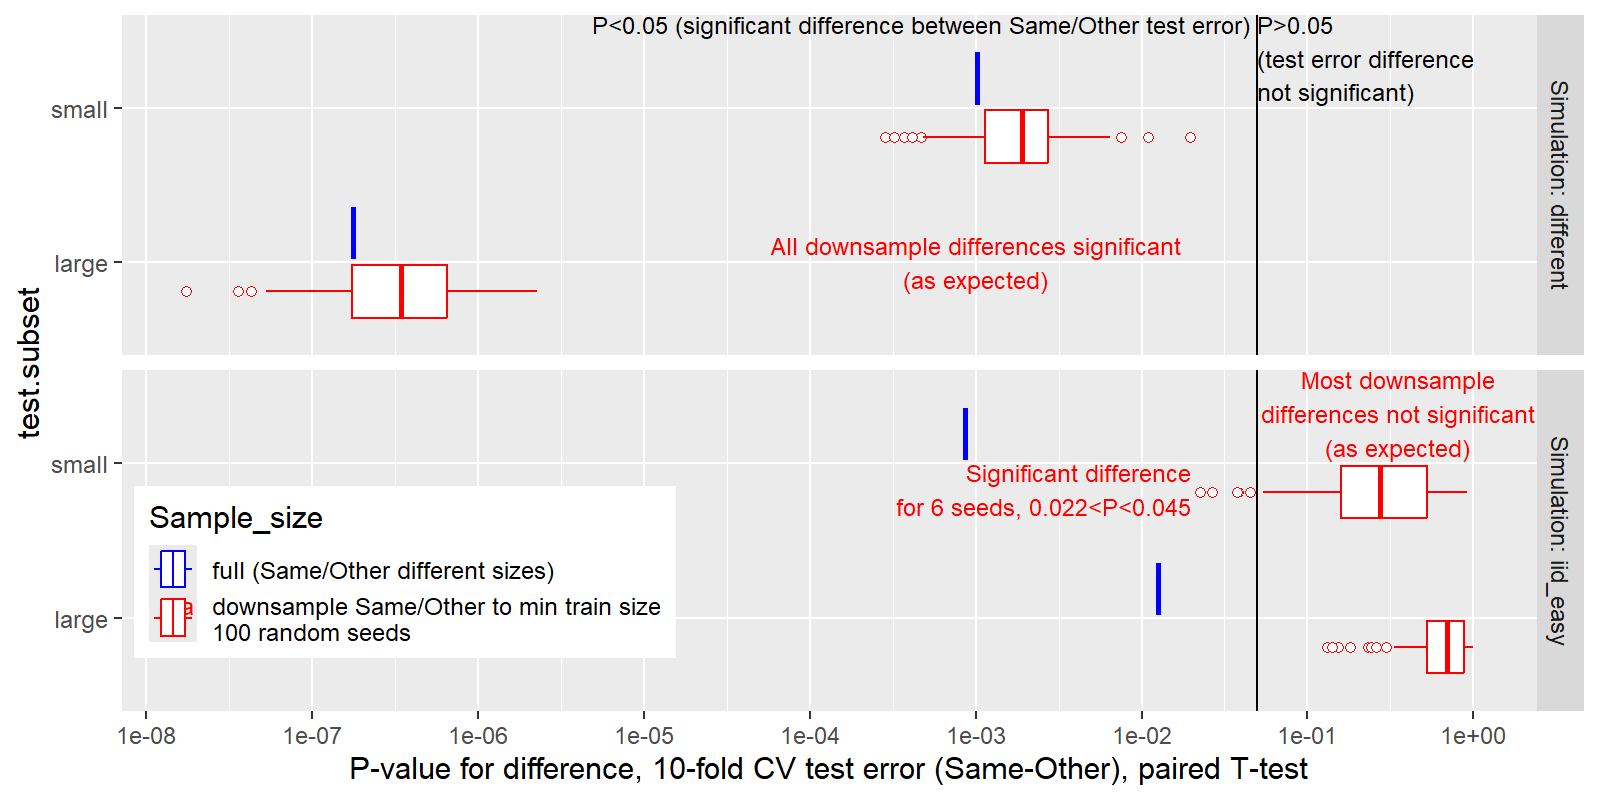
\includegraphics[width=0.8\textwidth]{fig3-simulations.png}
    \caption{Robustness of proposed SOKED evaluation framework, over 100 downsampling seeds in simulations (\texttt{different} and \texttt{iid\_easy}), using the rpart learner. Blue shows the full-data Same--Other p-value; boxes show matched-size p-values across seeds.}
    \label{fig:sim-combined}
\end{figure}

\subsection{Real regression data sets}
We next consider the three real regression examples, beginning with the traffic data because it motivates the learner choice used in the remaining regression experiments.

On the traffic data, we assessed whether the SOKED conclusion depends strongly on the prediction algorithm by comparing featureless, regression tree (\texttt{rpart}), elastic net (\texttt{glmnet}), and a torch-based multi-layer perceptron (MLP).
These learners span increasing model flexibility: the featureless learner predicts the training-set mean and serves as a no-signal baseline in \texttt{mlr3} \citep{Bischl2024}; \texttt{rpart} implements CART-style regression trees \citep{Breiman1984}; \texttt{glmnet} fits a cross-validated elastic-net generalized linear model \citep{Friedman2010glmnet}; and the MLP is a nonlinear neural network implemented with the R \texttt{torch} package \citep{rtorch}.
Figure~\ref{fig:learner-panels} focuses on the Phoenix test subset and reports test RMSE (mean $\pm$ SD across 5 CV splits) for the Same and Other train-subset configurations, both with the full available training sets and after matching both train sizes to the smaller feasible size.

\begin{figure}
    \centering
    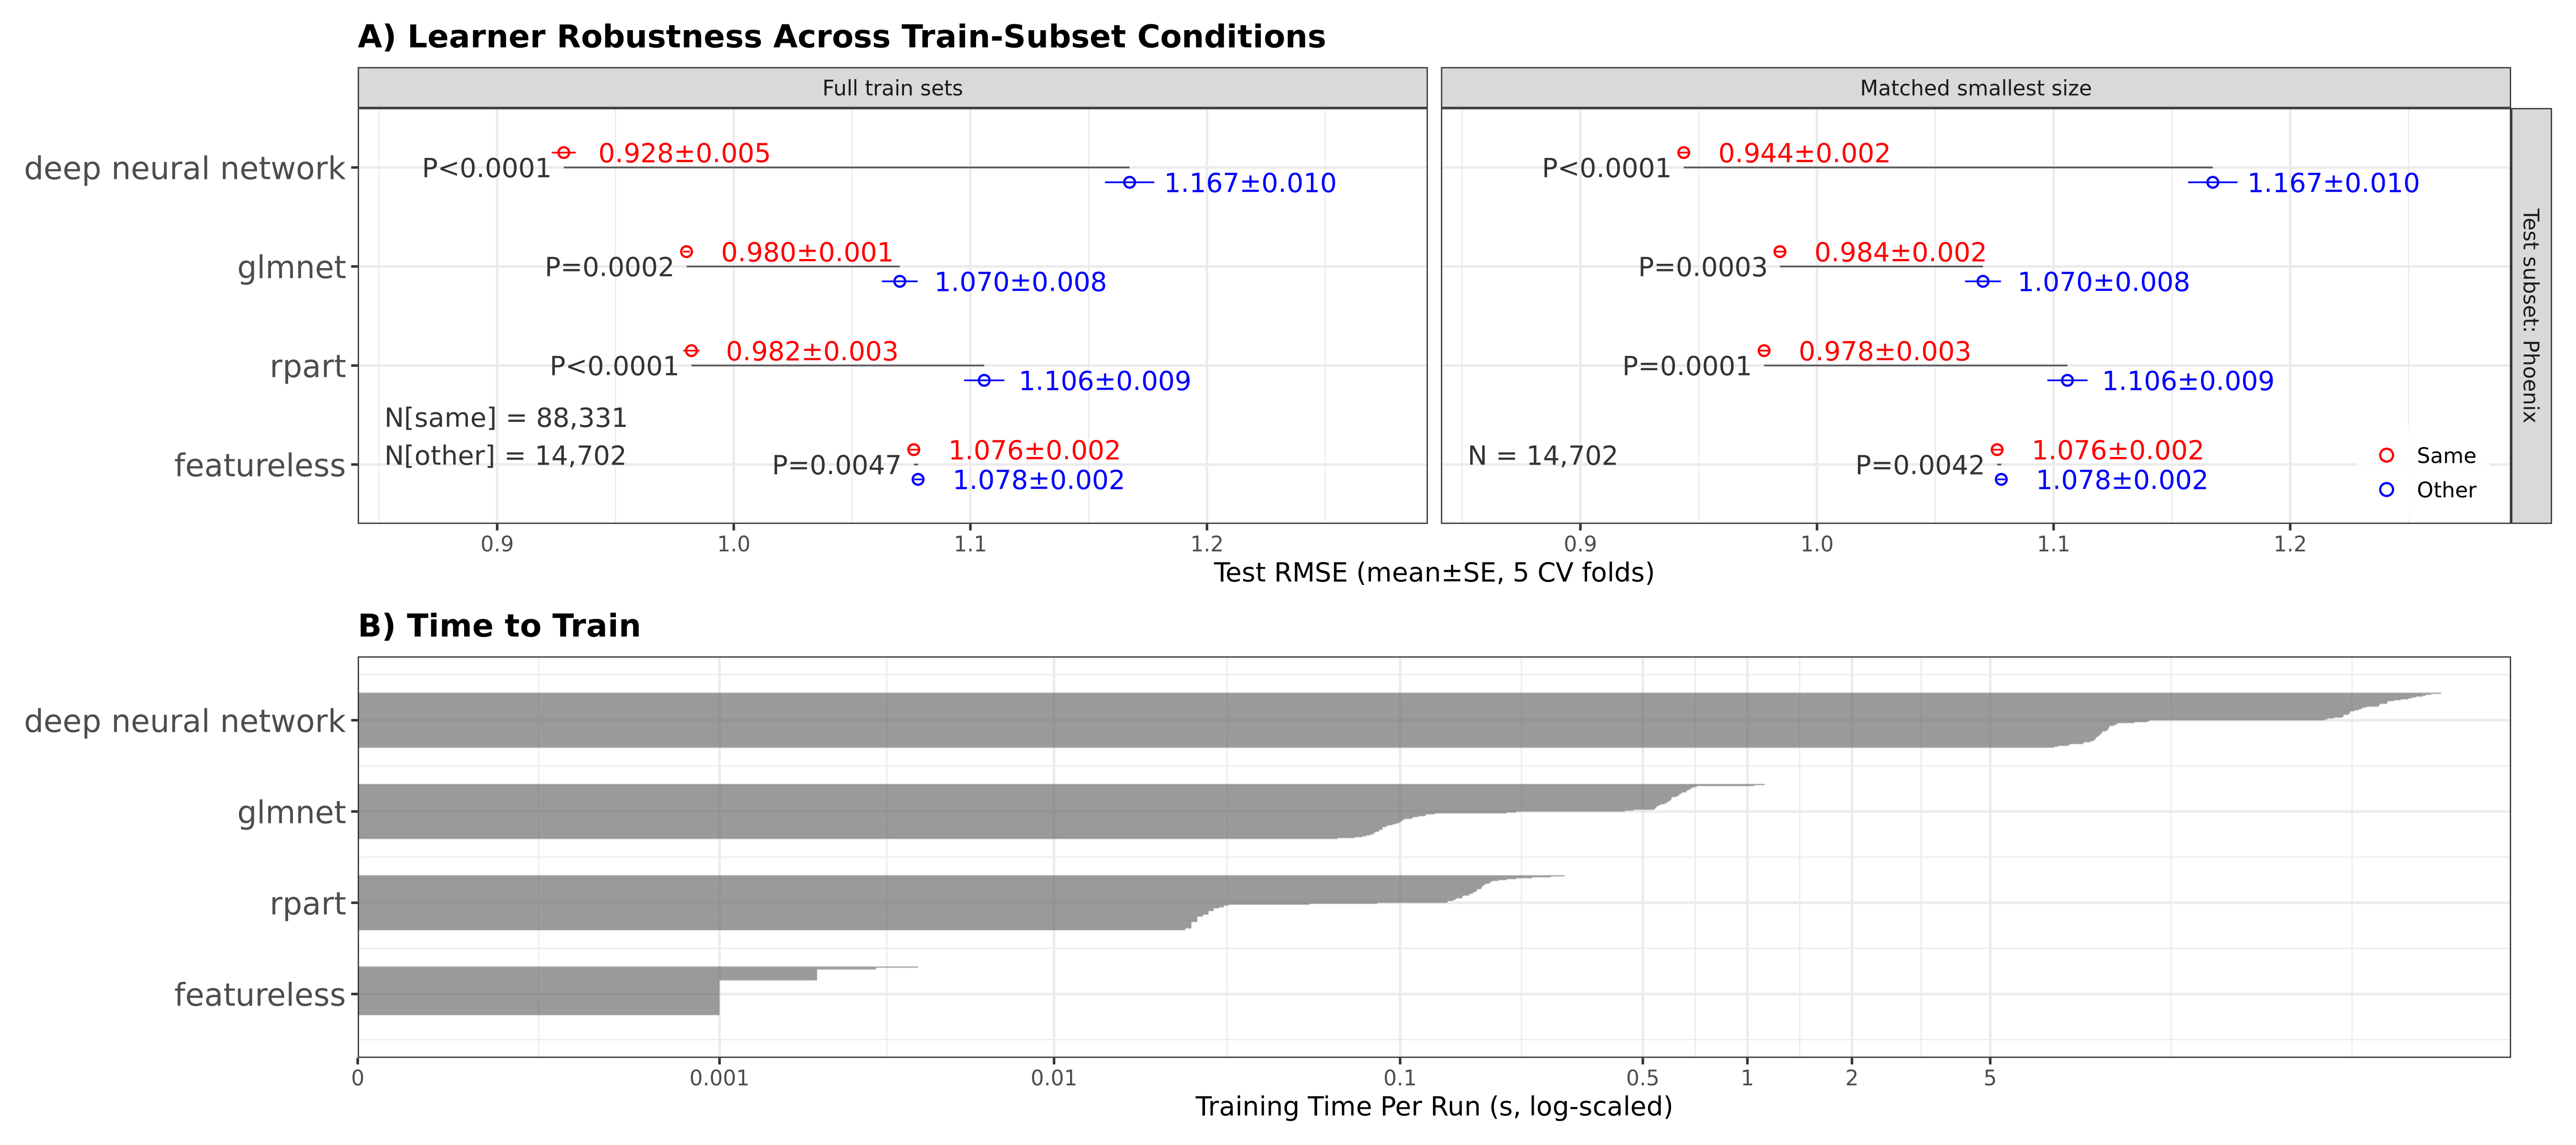
\includegraphics[width=\textwidth]{fig2-learner-panels.png}
    \caption{Learner robustness under SOKED (Phoenix test subset) on traffic data, comparing Same and Other at full and matched training sizes.}
    \label{fig:learner-panels}
\end{figure}

The qualitative SOKED conclusion is stable across the retained learner families in this example: training on the same subset is consistently better than training on the opposite subset, even after train-size matching.
With matched train size ($N=14{,}702$), Same improves over Other for every learner, from 1.076 against 1.078 for the featureless baseline to 0.944 against 1.167 for the torch MLP.
Among the non-featureless learners, \texttt{rpart} and \texttt{glmnet} both remain well below the featureless baseline in the matched-size condition, while the torch MLP gives the lowest RMSE.
With the full Phoenix-size Same training set ($N=88{,}331$), the strongest RMSE among the plotted learners comes from the torch MLP (0.928), followed by \texttt{glmnet} (0.980) and \texttt{rpart} (0.982).

% Panel B shows that these predictive gains come with large differences in computational cost.
% Featureless, \texttt{rpart}, and \texttt{glmnet} train in approximately 0.002, 0.12, and 0.44 seconds per run, respectively, whereas the tuned torch MLP requires about 32.2 seconds.
% Because the main SOKED diagnosis is stable across these learner families, we use \texttt{rpart} in the remaining experiments as a simple nonlinear default that is much cheaper than the neural network, substantially cheaper than \texttt{glmnet}, and still captures the same subset-dependent structure.

For qSIP, Figure~\ref{fig:regr-pairs} (middle column) shows SOKED results for the \texttt{qme.15} test subset.
At full training sizes, Same ($N=4{,}131$, RMSE $=0.0377$) outperforms Other ($N=2{,}808$, RMSE $=0.0564$), so the naive comparison could be attributed to Same having more training examples.
After downsampling Same to $n_0 = 2{,}808$, the gap persists (Same $0.0381$ vs.\ Other $0.0564$, $p < 0.0001$), confirming a strong residual subset effect.

For workers' compensation, Figure~\ref{fig:regr-pairs} (right column) shows the Female test subset.
At full training sizes, Other ($N=69{,}454$) outperforms Same ($N=20{,}545$) in RMSE ($1.741$ vs.\ $1.753$, $p < 0.0001$).
After downsampling to $n_0 = 20{,}545$, the gap narrows substantially (Other $1.748$ vs.\ Same $1.753$) and is no longer significant ($p = 0.117$).
This is the sample-size pattern SOKED is designed to reveal: most of the apparent full-data advantage of Other is explained by its larger training set rather than by a strong residual subset effect.

\begin{figure}
    \centering
    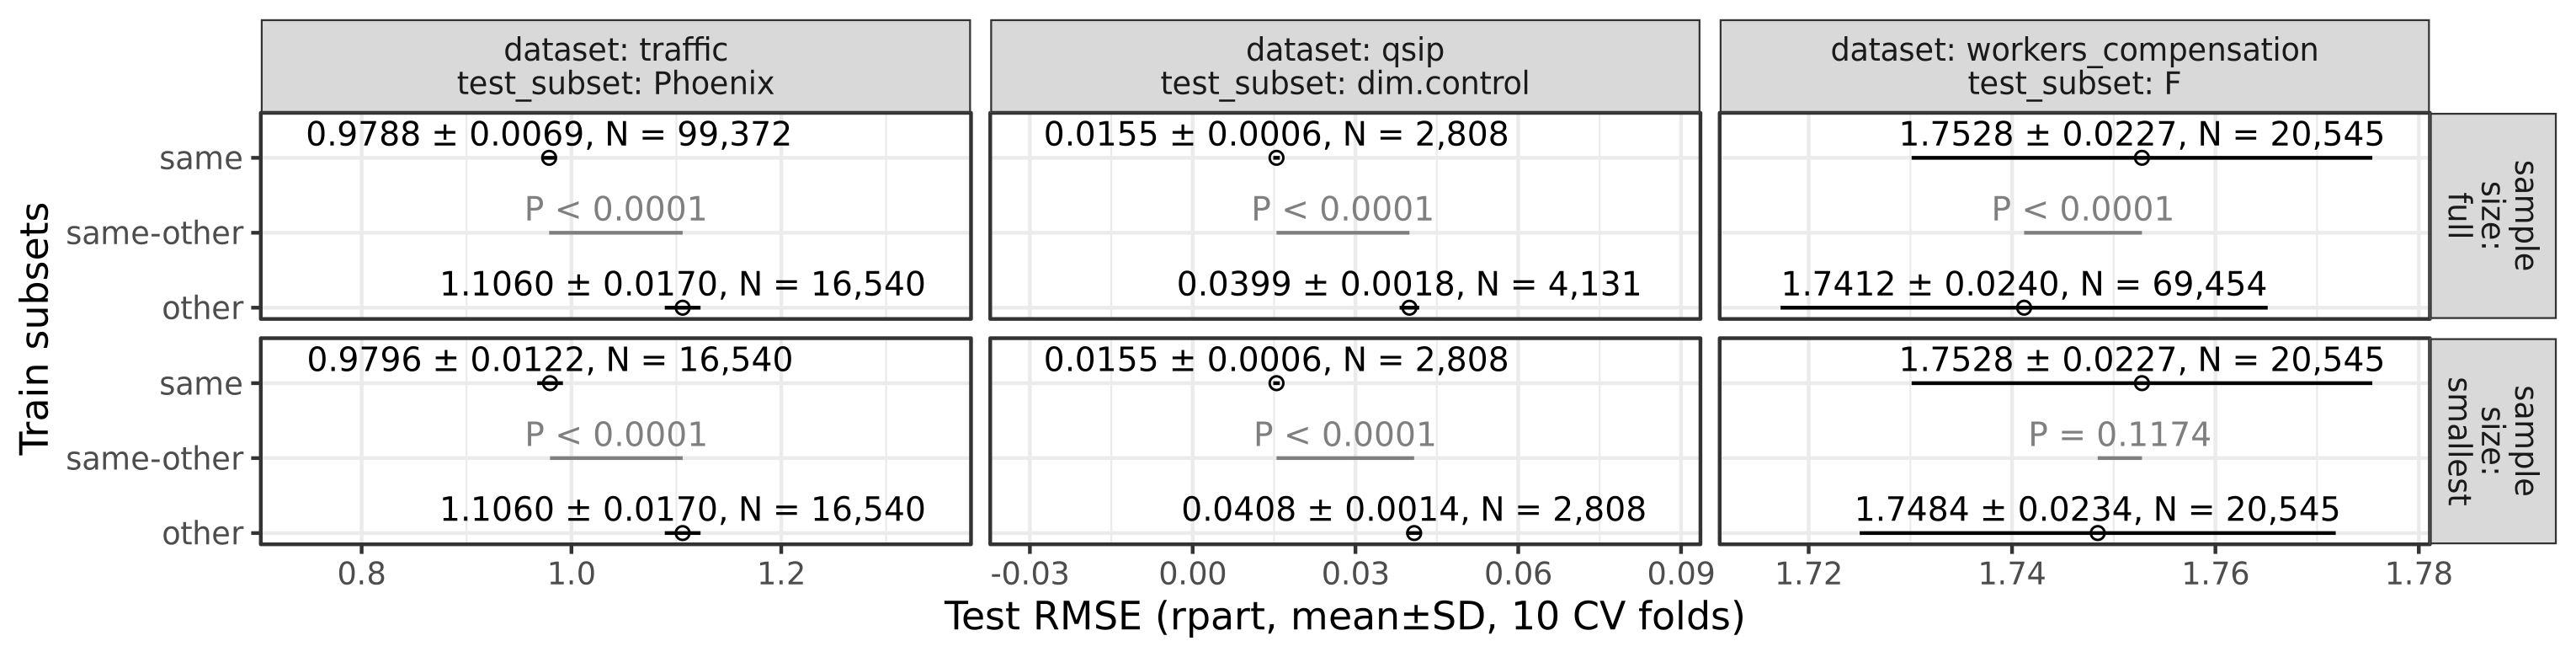
\includegraphics[width=\textwidth]{fig5-regr-pairs.png}
    \caption{
    SOKED results for three regression datasets (rpart learner, 10-fold CV), comparing Same and Other at full and matched training sizes by target subset.
    Each column corresponds to one dataset--test-subset pair.}
    \label{fig:regr-pairs}
\end{figure}

\subsection{Real classification data sets}
We then turn to the three real classification examples, which all use the same \texttt{glmnet} baseline but differ in whether the apparent advantage of Same or Other survives size matching.

For NSCH autism, Figure~\ref{fig:classif-pairs} (left column) shows SOKED results for the 2020 test subset.
The full-data comparison favors Same ($N=25{,}027$, error $= 0.0241$) over Other ($N=16{,}381$, error $= 0.0256$), and the gap is significant ($p = 0.0035$).
After downsampling to $n_0 = 16{,}381$, the gap narrows but does not disappear: Same still has lower error than Other ($0.0246$ vs.\ $0.0256$), and the matched-size gap remains significant ($p = 0.0126$).
This indicates a modest residual year-specific subset effect in addition to the sample-size advantage.
For the 2019 test subset (not shown), the pattern is different: Other is better at full size because it has more data, but the matched-size gap is non-significant ($p > 0.8$), which is consistent with a sample-size effect.
Taken together, NSCH shows both regimes across years: 2020 retains a small residual subset effect, whereas 2019 is largely explained by unequal sample sizes.

For STL-10, Figure~\ref{fig:classif-pairs} (middle column) shows SOKED results for the test-split target.
At full training sizes, Same ($N=7{,}200$, error $= 0.627$) outperforms Other ($N=4{,}500$, error $= 0.644$), and the gap is significant ($p = 0.0009$).
After downsampling to $n_0 = 4{,}500$, the gap narrows and becomes non-significant ($p = 0.193$), consistent with a sample-size effect.
When the training split is the target (not shown), Other is better at full size, but the matched-size gap is also non-significant ($p = 0.693$), again consistent with a sample-size effect rather than a strong residual subset difference.
In the current STL-10 runs, both target splits therefore behave primarily as sample-size examples.

For Waveform, Figure~\ref{fig:classif-pairs} (right column) shows SOKED results for the train-split target.
At full training sizes, Other ($N=450$, error $= 0.160$) outperforms Same ($N=270$, error $= 0.203$), with a modest but significant gap ($p = 0.046$).
After downsampling to $n_0 = 270$, the gap narrows substantially: Other rises to $0.193$ while Same remains at $0.203$, and the matched-size comparison is non-significant ($p = 0.533$).
For this target split, the apparent advantage of training on the Other subset is therefore largely explained by its larger training size rather than by a strong residual subset effect.
When the test split is the target (not shown), the gap likewise collapses after size-matching.
Taken together, Waveform behaves primarily as a sample-size example, and in the current STL-10 runs the same is true for both target splits.

\begin{figure}
    \centering
    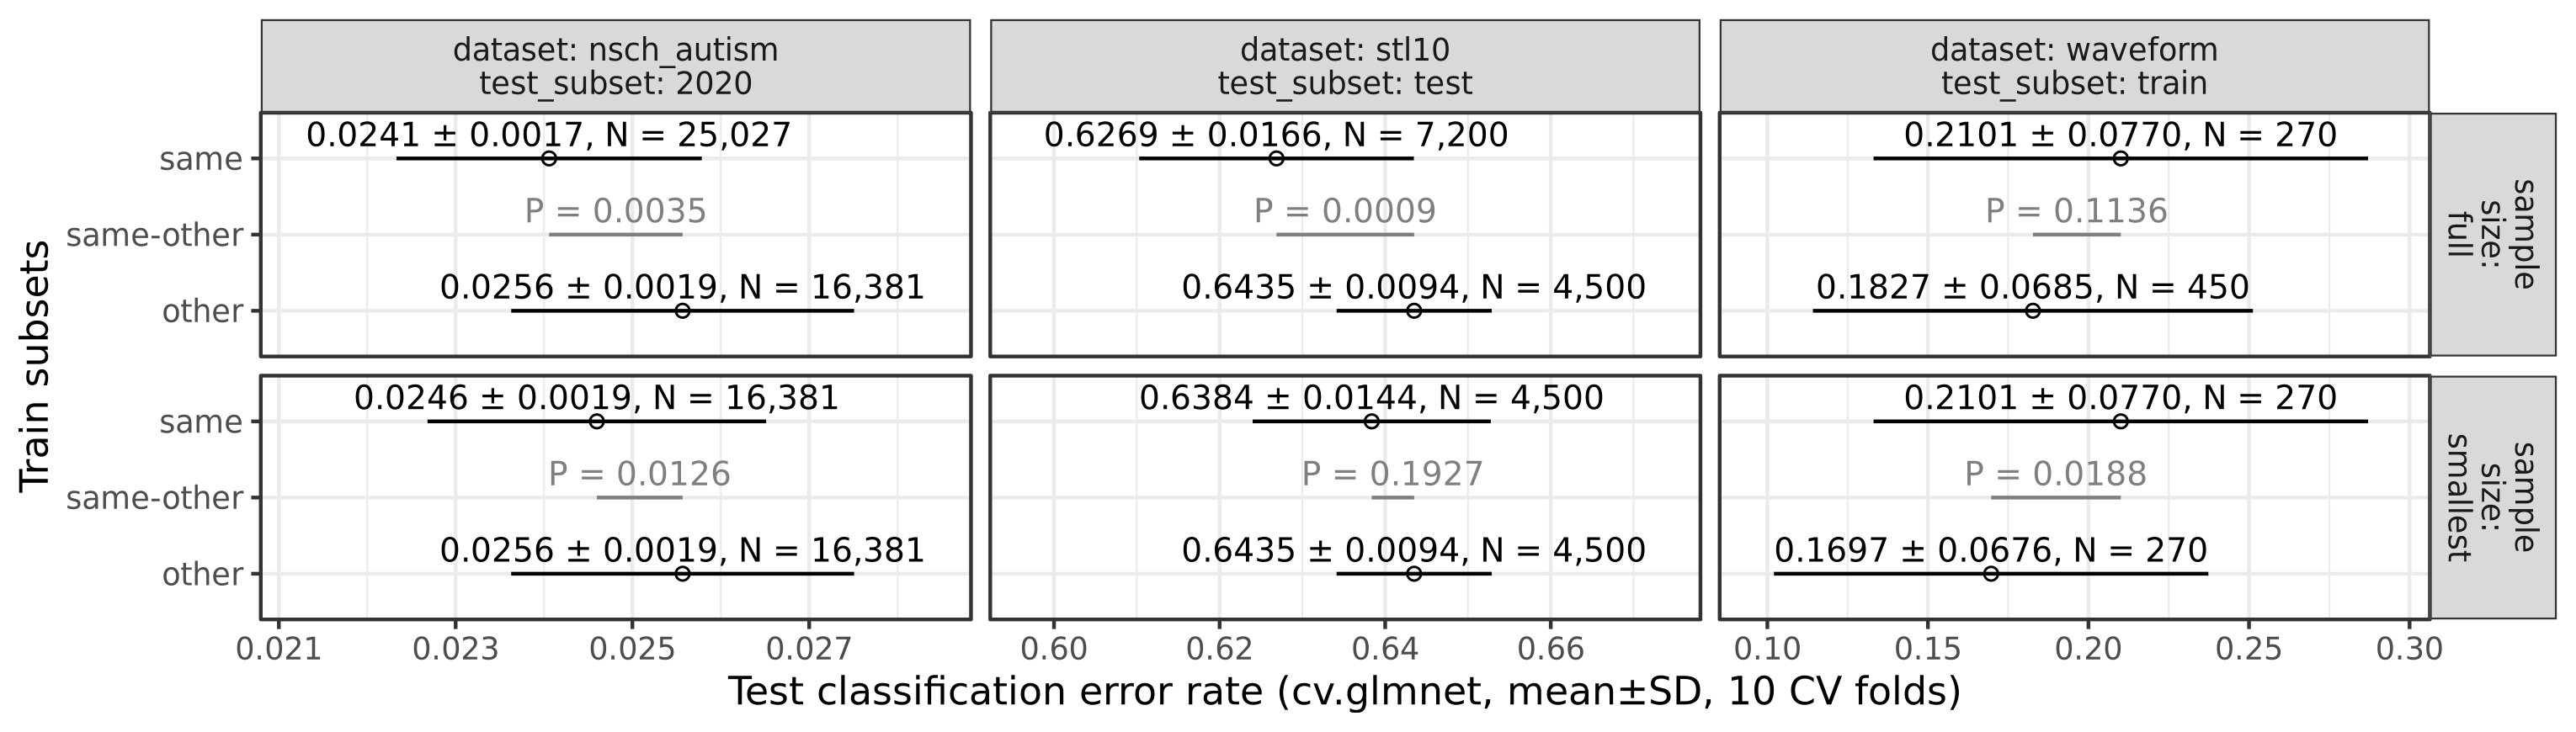
\includegraphics[width=\textwidth]{fig4-classif-pairs.png}
    \caption{
    SOKED results for three classification datasets (glmnet learner, 10-fold CV), comparing Same and Other at full and matched training sizes by target subset.
    Each column corresponds to one dataset--test-subset pair.}
    \label{fig:classif-pairs}
\end{figure}

\subsection{Summary of results across all data sets}
Table~\ref{tab:results-summary} consolidates the per-dataset findings into a single view that reports which source performs better before and after matching, along with which source is larger.
The scenario code is intentionally simple: O means Other is larger and also wins before matching, S means Same is larger and also wins before matching, and D means the smaller source already wins before matching.
The matched column is reported relative to the Larger column: \emph{larger} means the larger source still wins after matching, \emph{smaller} means the smaller source wins after matching, \emph{equal} means no matched-size winner, and \emph{n/a} means matching is not needed for interpretation.
For interpreted matched rows, the second line reports the paired $t$-test $p$-value for the matched-size Same--Other gap.
Of the 16 dataset/test-subset rows, 8 yield a residual subset effect that survives downsampling and 8 collapse to a sample-size effect, illustrating that both regimes occur in practice rather than one dominating.
The O and S rows are the ones SOKED actively resolves: they are exactly the cases where the larger source could be winning either because it is larger or because it is genuinely more predictive.
The D rows are already informative before downsampling because the smaller source wins outright, so matched-size downsampling is not needed for interpretation; those rows are therefore marked n/a in the matched column.
% The workers' comp / Female row remains especially consequential: the naive full-data comparison favors Other, but the matched-size comparison collapses to near-equality. This is the ordering reversal characterized by Proposition~\ref{prop:reversal}.

\begin{table}
    \centering
    \small
    \resizebox{\linewidth}{!}{%
    \begin{tabular}{lllcccll}
\toprule
Data &  Test subset & Algorithm & Better & Larger & Scenario & Better (matched) & Conclusion \\
\midrule
iid\_easy & small & rpart & other & other & O & \shortstack{equal\\($p=0.0992$)} & sample size \\
iid\_easy & large & rpart & other & same & D & n/a & sample size  \\
different & small & rpart & same & other & D & n/a & subset \\
different & large & rpart & same & same & S & \shortstack{larger\\($p=0.0009$)} & subset  \\
\midrule
qSIP & qme.15 & rpart & same & same & S & \shortstack{larger\\($p<0.0001$)} & subset \\
qSIP & dim.control & rpart & same & other & D & n/a & subset \\
workers' comp & Male & rpart & same & same & S & \shortstack{larger\\($p<0.0001$)} & subset \\
workers' comp & Female & rpart & other & other & O & \shortstack{equal\\($p=0.1174$)} & sample size \\
traffic & Phoenix & rpart & same & same & S & \shortstack{larger\\($p<0.0001$)} & subset \\
traffic & Baltimore & rpart & same & other & D & n/a & subset \\
\midrule
NSCH\_autism & 2019 & glmnet & other & other & O & \shortstack{equal\\($p=0.8168$)} & sample size \\
NSCH\_autism & 2020 & glmnet & same & same & S & \shortstack{larger\\($p=0.0126$)} & subset \\
STL-10 & test & glmnet & same & same & S & \shortstack{equal\\($p=0.1927$)} & sample size \\
STL-10 & train & glmnet & other & other & O & \shortstack{equal\\($p=0.6931$)} & sample size \\
Waveform & test & glmnet & same & same & S & \shortstack{equal\\($p=0.8542$)} & sample size \\
Waveform & train & glmnet & other & other & O & \shortstack{equal\\($p=0.5325$)} & sample size \\
\bottomrule
\end{tabular}}
    \caption{SOKED results across all datasets.
    }
    \label{tab:results-summary}
\end{table}

\section{Conclusion}
We introduced SOKED, a framework that extends Same/Other cross-validation with matched-size downsampling to formally decompose observed performance gaps into a sample-size component and a residual subset component.
The decomposition is operationally simple: run the Same/Other comparison twice (once at full training sizes and once with the larger configuration downsampled to the smaller feasible size) and compare the two results.
If the gap collapses after matching, it is a sample-size effect and the remedy is more data collection.
If the gap persists, it is a genuine subset effect and the remedy is distributional robustness or domain adaptation.

Across six real and two simulated datasets spanning regression and classification, image recognition, survey epidemiology, microbial biogeochemistry, and insurance claims, SOKED consistently distinguished these two causes.
Several rows, including NSCH autism 2019, both STL-10 rows, both Waveform rows, and workers' compensation Female, lose their apparent advantage after size-matching, pointing to data collection as the right response in those settings.
Other rows, including traffic, qSIP, workers' compensation Male, and NSCH autism 2020, retain a matched-size gap, indicating genuine distributional differences between subsets.
For the workers' compensation Female experiment, the naive full-data comparison favors Other, while SOKED reveals that this apparent advantage shrinks to a non-significant difference once sizes are equalized.

The seed-robustness experiment on simulated data confirms that the SOKED conclusion is stable across 100 random downsampling seeds, supporting practical use of a single seed when compute is limited.
The learner-robustness experiment on the traffic dataset confirms that the Same-beats-Other conclusion holds across different models, at the cost of substantially increasing training time for more expressive models.

SOKED is implemented in the \texttt{mlr3resampling} R package and integrates with the full \texttt{mlr3} benchmarking ecosystem.
Future work includes extending the downsampling strategy to pooled training configurations to further isolate complementarity effects, and developing power analysis tools to guide the choice of number of folds and downsampling seeds.

\paragraph{Limitations.}
The decomposition is operational rather than causal: a persistent matched-size gap is evidence against exchangeability but does not identify which distributional factor drives it.
SOKED always matches at the minimum training size, the most conservative choice; when one subset is very large, this discards substantial data and reduces statistical power.
As discussed in Section~\ref{sec:ttest}, the reported $p$-values are diagnostic summaries of fold-level gaps, not exact inferential guarantees; SOKED conclusions should therefore be read together with the observed direction and magnitude of the matched-size gaps.
Finally, SOKED inherits the computational cost of running benchmark experiments at two training sizes; for expensive learners such as deep neural networks, this may be prohibitive.

\begin{ack}
% Acknowledgments omitted for blind review. 
%  TODO
\end{ack}

\bibliographystyle{abbrvnat}
\bibliography{refs}

\appendix
\section{Proofs}
\label{app:proofs}

\begin{proof}[Proof of Lemma~\ref{lem:exchangeability}]
Under the stated conditions, the joint distribution of $(X_i, Y_i)$ is the same for observations drawn from subset $a$ as for those drawn from subset $b$.
Given $n_0$ training examples, the predictors $\hat{h}_{a,n_0}$ and $\hat{h}_{b,n_0}$ therefore have the same distribution over the randomness of the training draw.
It follows that $\mathbb{E}[L_t(\hat{h}_{a,n_0})] = \mathbb{E}[L_t(\hat{h}_{b,n_0})]$, giving $\mathbb{E}[\Delta_t^{\mathrm{match}}(a,b)] = 0$.
\end{proof}

\begin{proposition}[Characterization of ordering reversal]
\label{prop:reversal}
Let $f_c(n) = \mathbb{E}[L_t(\hat{h}_{c,n})]$ and suppose $n_b \geq n_a$, so $n_0 = n_a$.
Let $\delta_q := f_b(n_0) - f_a(n_0)$ be the quality advantage of $a$ at matched size, and $\delta_s := f_b(n_0) - f_b(n_b) \geq 0$ be the size gain of $b$.
Then $\mathbb{E}[\Delta_t^{\mathrm{match}}] = -\delta_q$ and $\mathbb{E}[\Delta_t^{\mathrm{full}}] = \delta_s - \delta_q$.
Ordering reversal occurs if and only if $0 < \delta_q < \delta_s$: $a$ is the better source at matched size, but $b$'s size advantage is large enough to overcome that quality deficit.
If $\delta_s = 0$, reversal is impossible and SOAK suffices; if $\delta_q = 0$, the gap is a pure sample-size effect.
\end{proposition}

\begin{proof}[Proof of Proposition~\ref{prop:reversal}]
By definition, $\mathbb{E}[\Delta_t^{\mathrm{match}}(a,b)] = f_a(n_0) - f_b(n_0) = -\delta_q$.
For the full-data gap, $\mathbb{E}[\Delta_t^{\mathrm{full}}(a,b)] = f_a(n_a) - f_b(n_b) = f_a(n_0) - f_b(n_b)$ (since $n_a = n_0$).
Adding and subtracting $f_b(n_0)$ gives $f_a(n_0) - f_b(n_0) + f_b(n_0) - f_b(n_b) = -\delta_q + \delta_s = \delta_s - \delta_q$.
Ordering reversal requires $\Delta_t^{\mathrm{match}}$ and $\Delta_t^{\mathrm{full}}$ to have opposite signs, i.e., $(-\delta_q)(\delta_s - \delta_q) < 0$, which holds iff $0 < \delta_q < \delta_s$.
\end{proof}

\section*{NeurIPS Paper Checklist}

\begin{enumerate}

\item {\bf Claims}
    \item[] Question: Do the main claims made in the abstract and introduction accurately reflect the paper's contributions and scope?
    \item[] Answer: \answerYes{}
    \item[] Justification: The abstract and introduction state four concrete contributions: (1) a formal decomposition of performance gaps into sample-size and subset components, (2) the SOKED algorithm, (3) the ordering-reversal failure mode, and (4) empirical demonstrations across nine datasets. All four are delivered in the paper.

\item {\bf Limitations}
    \item[] Question: Does the paper discuss the limitations of the work performed by the authors?
    \item[] Answer: \answerYes{}
    \item[] Justification: The Conclusion section notes that SOKED matches at the minimum training size (the most conservative choice), and that future work is needed for power analysis to guide the number of folds and downsampling seeds. The decomposition is operational rather than causal, and this is acknowledged in Section~3.1.

\item {\bf Theory assumptions and proofs}
    \item[] Question: For each theoretical result, does the paper provide the full set of assumptions and a complete (and correct) proof?
    \item[] Answer: \answerYes{}
    \item[] Justification: Lemma~1 and Proposition~1 state all assumptions explicitly. Full proofs are provided in Appendix~A.

\item {\bf Experimental result reproducibility}
    \item[] Question: Does the paper fully disclose all the information needed to reproduce the main experimental results of the paper to the extent that it affects the main claims and/or conclusions of the paper (regardless of whether the code and data are provided or not)?
    \item[] Answer: \answerYes{}
    \item[] Justification: Section~3.3 specifies the learner, number of CV folds, number of downsampling seeds, and matched training size $n_0$ for each dataset. SOKED is implemented in the publicly available \texttt{mlr3resampling} R package.

\item {\bf Open access to data and code}
    \item[] Question: Does the paper provide open access to the data and code, with sufficient instructions to faithfully reproduce the main experimental results, as described in supplemental material?
    \item[] Answer: \answerYes{}
    \item[] Justification: The SOKED framework is implemented in the \texttt{mlr3resampling} R package (available on CRAN). STL-10, UCI Waveform, and NSCH are publicly available datasets. The workers' compensation dataset is publicly available via the cited source. Experiment scripts are available in the supplemental material.

\item {\bf Experimental setting/details}
    \item[] Question: Does the paper specify all the training and test details (e.g., data splits, hyperparameters, how they were chosen, type of optimizer) necessary to understand the results?
    \item[] Answer: \answerYes{}
    \item[] Justification: Section~3.3 reports the learner, number of CV folds ($B=5$ or $B=10$), number of downsampling seeds ($R=1$ or $R=100$), and matched training size for each experiment. Learners use default hyperparameters from \texttt{mlr3}.

\item {\bf Experiment statistical significance}
    \item[] Question: Does the paper report error bars suitably and correctly defined or other appropriate information about the statistical significance of the experiments?
    \item[] Answer: \answerYes{}
    \item[] Justification: All figures report mean $\pm$ SD or mean $\pm$ SE across CV folds. Paired $t$-test $p$-values comparing Same vs.\ Other at matched training size are reported for every dataset, with the test procedure described in Section~3.2.

\item {\bf Experiments compute resources}
    \item[] Question: For each experiment, does the paper provide sufficient information on the computer resources (type of compute workers, memory, time of execution) needed to reproduce the experiments?
    \item[] Answer: \answerYes{}
    \item[] Justification: Figure~2 (Panel B) reports per-run training time for each learner on the traffic dataset. Experiments were run on a SLURM HPC cluster; individual job resource requirements (walltime 2h, memory 24GB) are specified in the supplemental scripts.

\item {\bf Code of ethics}
    \item[] Question: Does the research conducted in the paper conform, in every respect, with the NeurIPS Code of Ethics?
    \item[] Answer: \answerYes{}
    \item[] Justification: The paper uses only publicly available datasets and introduces a diagnostic methodology. No data was collected from human subjects by the authors. The NSCH autism data is an anonymized public survey; the workers' compensation data is synthetic.

\item {\bf Broader impacts}
    \item[] Question: Does the paper discuss both potential positive societal impacts and negative societal impacts of the work performed?
    \item[] Answer: \answerYes{}
    \item[] Justification: The paper explicitly discusses fairness auditing as a use case (Related Work and workers' compensation experiment): SOKED separates sample-size effects from genuine distributional differences, which has positive implications for equitable model evaluation across demographic groups. No significant negative societal impact is anticipated for a model evaluation methodology.

\item {\bf Safeguards}
    \item[] Question: Does the paper describe safeguards that have been put in place for responsible release of data or models that have a high risk for misuse?
    \item[] Answer: \answerNA{}
    \item[] Justification: The paper introduces a cross-validation methodology and releases no new datasets or generative models that pose misuse risks.

\item {\bf Licenses for existing assets}
    \item[] Question: Are the creators or original owners of assets used in the paper properly credited and are the license and terms of use explicitly mentioned and properly respected?
    \item[] Answer: \answerYes{}
    \item[] Justification: All datasets are cited: STL-10 \citep{coates2011stl10}, UCI Waveform \citep{breiman1984classification}, workers' compensation \citep{Ali2020}, NSCH (U.S.\ Census Bureau public-use file), traffic and qSIP (cited co-authors). The \texttt{mlr3resampling} package is MIT-licensed.

\item {\bf New assets}
    \item[] Question: Are new assets introduced in the paper well documented and is the documentation provided alongside the assets?
    \item[] Answer: \answerYes{}
    \item[] Justification: The primary new asset is the SOKED implementation in \texttt{mlr3resampling}, which is documented on CRAN with vignettes and a function reference. The \texttt{ResamplingSameOtherSizesCV} class and \texttt{pvalue\_downsample()} function implement the methods described in Sections~3.1--3.2.

\item {\bf Crowdsourcing and research with human subjects}
    \item[] Question: Does the paper include the full text of instructions given to participants and screenshots, if applicable, as well as details about compensation?
    \item[] Answer: \answerNA{}
    \item[] Justification: The paper does not involve crowdsourcing or direct research with human subjects. The NSCH dataset is a pre-existing public survey conducted by the U.S.\ Census Bureau.

\item {\bf Institutional review board (IRB) approvals or equivalent for research with human subjects}
    \item[] Question: Does the paper describe potential risks incurred by study participants and whether IRB approvals were obtained?
    \item[] Answer: \answerNA{}
    \item[] Justification: No human subjects research was conducted by the authors. The NSCH autism dataset is a de-identified public-use file; the workers' compensation dataset is synthetic.

\item {\bf Declaration of LLM usage}
    \item[] Question: Does the paper describe the usage of LLMs if it is an important, original, or non-standard component of the core methods in this research?
    \item[] Answer: \answerNA{}
    \item[] Justification: LLMs were not used as part of the core methodology, algorithms, or experimental design.

\end{enumerate}


\end{document}
